\subsubsection{Auslegung Schwungradantrieb}
\label{BestimmungDrehmomentSchwundrad}
Um den Schwungradantrieb auslegen zu können werden Nenndrehzahl und Nenndrehmoment 
benötigt. Diese werden nachfolgende anhand zwei unterschiedlichen Ansätzen berechnet.
Der eine Ansatz ist über das Quetschen des Balles und der Andere ist über die 
Energieerhaltung.
%
\paragraph{Momenterzeugung durch Quetschen des Balles}$~~$\vspace{2mm}\\
In der Tabelle \ref{tab:glossarQuetschen} sind die benötigten Formelzeichen und 
deren Bedeutung aufgelistet, die für die Berechnung mit dem Quetschansatz benötigt 
werden.
\begin{table}[h!]
    \begin{tabular}{lcl}
        \rule{0pt}{11pt}Zeichen & Einheit & Bezeichnung \\
        \hline\rule{0pt}{11pt}$F_S$ & $N$ & Kraft für das Stauchen des Balles \\
        \rule{0pt}{11pt}$k$ & $\frac{N}{m}$ & Federkonstante Ball \\
        \rule{0pt}{11pt}$\Delta x$ & $m$ & Federweg \\
        \rule{0pt}{11pt}$g$ & $\frac{N}{kg}$ & Erdgravitation \\
        \rule{0pt}{11pt}$m_L$ & $kg$ & Lastgewicht \\
        \rule{0pt}{11pt}$d_s$ & $m$ & Durchmesser maximal gestauchter Ball \\
        \rule{0pt}{11pt}$d_B$ & $m$ & Durchmesser Tennisball (Normalzustand) \\
        \rule{0pt}{11pt}$s_{max}$ & $m$ & maximaler Federweg pro Seite \\
        \rule{0pt}{11pt}$L_a$ & $m$ & Abstand zwischen Schwungräder \\
        \rule{0pt}{11pt}$R_S$ & $m$ & Radius des Schwungrades \\
        \rule{0pt}{11pt}$\alpha_{Grenz}$ & $^\circ Grad$ & Winkel während dem der Ball gestaucht wird \\
        \rule{0pt}{11pt}$M_S$ & $Nm$ & Moment welches auf das Schwungrad wirkt \\
        \rule{0pt}{11pt}$F_t$ & $N$ & Torsionskraft \\
        \rule{0pt}{11pt}$\alpha$ & $^\circ Grad$ & Kontaktwinkel zwischen Schwungrad und Ball \\
        \rule{0pt}{11pt}$\Delta x(\alpha)$ & $m$ & Wegdifferenz bei Winkel $\alpha$ \\
        \rule{0pt}{11pt}$s(\alpha)$ & $m$ & Stauchung bei Winkel $\alpha$ \\
    \end{tabular}
        \centering
        \caption{Glossar für die Berechnung über das Quetschen des Balles}
        \label{tab:glossarQuetschen}
\end{table}

Damit der Ball mit einem Anpressdruck durch die Schwungräder beschleunigt 
wird, benötigt es ein Drehmoment. Als Grundlage dient die Annahme, dass sich der 
Ball wie eine Feder verhält.

\begin{figure}[h!]
    \centering
    \includegraphics[width=0.7\textwidth]
    {Enddokumentation/Anhang/Bilder/KompressionBaelle.jpg}
    \caption{Prinzip der $k$-Bestimmung}
    \label{fig:BallKomp}
\end{figure}

Aus einem Versuch, der wie in Abbildung \ref{fig:BallKomp} aufgebaut war, ergaben sich die in Tabelle \ref{tab:BallKompErgebnis} enthaltenen Messergebnisse. Aus diesen wird mit den Formeln \ref{equ:F_s} und \ref{equ:k} die Federkraft bestimmt. Diese verhält sich progressiv. Sie kann für die weitere Berechnung als linear angesehen werden, da die Auslenkung $\Delta x$ nicht sehr gross, und somit ist die Veränderungen der Federkonstante gering (kleiner $0.5 \frac{N}{mm}$).
\begin{align}  
    F_s &= k \cdot \Delta x 
    \label{equ:F_s}\\
    k &= \dfrac{m_L \cdot g}{\Delta x}
    \label{equ:k}
\end{align}
\begin{table}[h!]
    \begin{tabular}{ccc}
        \rule{0pt}{11pt} Masse $m$ $\left[kg\right]$ & Auslenkung $\Delta x 
        \left[mm\right]$ & Federkonstante $k \left[\frac{N}{mm}\right]$\\
        \hline
        \rule{0pt}{11pt} $1.025 kg$ & $1.02 mm$ & $9.86  \frac{N}{mm}$\\
        \rule{0pt}{11pt} $2.345 kg$ & $2.24 mm$ & $10.27 \frac{N}{mm}$\\
        \rule{0pt}{11pt} $3.485 kg$ & $3.25 mm$ & $10.52 \frac{N}{mm}$\\
    \end{tabular}
    \centering
    \caption{Messergebnisse und Berechnung der Federkonstante}
    \label{tab:BallKompErgebnis}
\end{table}

Für die weiteren Berechnungen wird eine Federkonstante von $10 \frac{N}{mm}$ 
verwendet. (vgl. Tabelle \ref{tab:BallKompErgebnis})\\
\\
Anhand trigonometrischer Beziehungen wird das Drehmoment, welches auf die 
Schwungräder wirkt berechnet (siehe nachfolgende Formeln). Dazu wird zunächst 
der Grenzwinkel $\alpha_{Grenz}$ bestimmt. Dies ist der Winkel, während dem der Ball 
gestaucht wird. Die Berechnung des Drehmomentes folgt über diesen Grenzwinkel. 
Dabei wirkt die Federkraft jeweils im Abwurfwinkel zu den Schwungrädern und 
ergibt das Drehmoment $M$, welches sich sinusförmig verhält. 
%
\begin{align}  
    s_{max} &= \frac{d_B - d_s}{2}\\
    L_a &= 2 \cdot R_s + d_s\\
    \alpha_{Grenz} &= \arccos\left(\frac{R_s - s_{max}}{R_s}\right)
\end{align}

\begin{figure}[h!]
    \centering
    \includegraphics[width=0.9\textwidth]{Enddokumentation/Anhang/Bilder/TrigoBeziehungen.jpg}
    \caption{Trigonometrische Beziehungen}
    \label{fig:trigoBeziehungen}
\end{figure}
\textbf{Berechnungswerte}\\
\begin{tabular}{lll}
    \rule{0pt}{11pt} $d_B$ & $68.6 mm$ & kleinster $(d_s)$ / grösster $(d_B)$ \\
    \rule{0pt}{11pt} $d_s$ & $65.4 mm$ & Tennisball nach Tennisregelwerk \\
    \rule{0pt}{11pt} $R_s$ & $40 mm$ & durch Konstruktion gegeben \\
\end{tabular}

\textbf{Resultate}\\
\begin{tabular}{ll}
    \rule{0pt}{11pt} $L_a$ & $145.5 mm$ \\
    \rule{0pt}{11pt} $s_{max}$ & $1.6 mm$ \\
    \rule{0pt}{11pt} $\alpha_{Grenz}$ & $16.26^\circ$ \\
\end{tabular}

\begin{figure}[h!]
    \begin{minipage}[hbt]{0.6\textwidth}
        \begin{align}  
            M_s &= R_S \cdot F_t \\
            F_t &= F_s \cdot \sin(\alpha) \\ 
            F_s &= 2\cdot k \cdot \Delta x \\
            \Delta x_{(\alpha)} &= s_{max} - s_{(\alpha)} \\
            s_{(\alpha)} &= R_s \cdot \left[1 - \cos(\alpha)\right]
        \end{align}
        Aus den obigen Formeln kann nun die Beziehung zwischen dem Moment, dem Winkel 
        $\alpha$ und dem Definitionsbereich von $-\alpha_{Grenz} \leq \alpha \leq  
        \alpha_{Grenz}$ hergestellt werden.        
        \begin{equation}  
            M_s = 2 \cdot R_s \cdot \sin(\alpha) \cdot \left(s_{max} - R_s \cdot \left[1 - 
            \cos(\alpha)\right]\right)
        \end{equation}
    \end{minipage}
\hfill
    \begin{minipage}[hbt]{0.45\textwidth}
        \includegraphics[scale=0.6,clip,trim=18mm 10mm 8mm 19mm]
        {Enddokumentation/Anhang/Bilder/Kraeftediagramm.jpg}
        \centering
        \caption{Kräftediagramm}
        \label{abb:Kraeftediagramm}
    \end{minipage}
\end{figure}
\vspace{1pt}
Aus dem grafischen Momentverlauf in Abbildung \ref{fig:momentverlauf} kann das maximal 
benötigte Drehmoment für das Quetschen des Balles herausgelesen werden. Dieses beträgt 
$13.7 Nmm$.

\begin{figure}[h!]
    \centering
    \includegraphics[width=1\textwidth,clip,trim=0mm 0mm 60mm 0mm]
    {Enddokumentation/Anhang/Bilder/Momentenverlauf.jpg}
    \caption{Momentverlauf}
    \label{fig:momentverlauf}
\end{figure}
\newpage
Da aufgrund experimenteller Versuche, die Schwungräder auch bei diesem vorhandenen 
Drehmoment sich abbremsten, kamen wichtige Erkenntnisse zum Vorschein. Der Motor 
reagiert relativ träge auf eine Laständerung. Deshalb steht das erforderliche Drehmoment 
nicht zur Verfügungen. Ein hohes Drehmoment bringt somit nur einen Zeitgewinn beim 
Beschleunigen der Räder auf ihre Nenndrehzahl mit sich.
%\newpage
%
\paragraph{Energiebilanzierung Ballwurf}$~~$\vspace{2mm}\\
In der Tabelle \ref{tab:glossarEnergie} sind die benötigten Formelzeichen und 
deren Bedeutung aufgelistet, die für die Berechnung mit der Energieerhaltung
benötigt werden.
\begin{table}[h!]
    \begin{tabular}{lcl}
    \rule{0pt}{11pt}Zeichen & Einheit & Bezeichnung \\
    \hline\rule{0pt}{11pt} $E_{pot}$ & $\frac{kgm^2}{s^2}$ & potentielle Energie des Balles \\
    \rule{0pt}{11pt}$E_{kin}$ & $\frac{kgm^2}{s^2}$	& kinetische Energie des Balles \\
    \rule{0pt}{11pt}$E_{rot}$ & $\frac{kgm^2}{s^2}$	& rotative Energie des Schwungrades \\
   	\rule{0pt}{11pt}$m_{Ball}$ & $kg$ & Masse Tennisball \\
   	\rule{0pt}{11pt}$h_0$ & $m$ & Höhenlage des Balles bei Punkt 0 \\
   	\rule{0pt}{11pt}$h_1$ & $m$ & Höhenlage des Balles bei Punkt 1 \\
   	\rule{0pt}{11pt}$\Delta h$ & $m$ & Höhenlagedifferenz $h_1 - h_0$ \\
   	\rule{0pt}{11pt}$v_0$ & $\frac{m}{s}$ & Geschwindigkeit des Balles in Punkt 0 \\
   	\rule{0pt}{11pt}$v_1$ & $\frac{m}{s}$ & Geschwindigkeit des Balles in Punkt 1 \\
   	\rule{0pt}{11pt}$v_{Band}$ & $\frac{m}{s}$ & Bandgeschwindigkeit der Ballzuführung \\
   	\rule{0pt}{11pt}$v_{u1}$ & $\frac{m}{s}$ & Umfangsgeschwindigkeit Schwungrad in Punkt 1 \\
   	\rule{0pt}{11pt}$\alpha_{Grenz}$ & $^\circ Grad$ & Grenzwinkel \\
   	\rule{0pt}{11pt}$\omega$ & $\frac{rad}{s^2}$ & Winkelbeschleunigung \\
   	\rule{0pt}{11pt}$\omega_0$ & $\frac{rad}{s}$ & Winkelgeschwindigkeit in Punkt 0 \\
   	\rule{0pt}{11pt}$\omega_1$ & $\frac{rad}{s}$ & Winkelgeschwindigkeit in Punkt 1 \\
   	\rule{0pt}{11pt}$J$ & $kgm^2$ & Trägheitsmoment des Schwungrades \\
   	\rule{0pt}{11pt}$R_s$ & $m$ & Radius des Schwungrades \\
   	\rule{0pt}{11pt}$n_0$ & $\frac{1}{s}$ & Nenndrehzahl in Punkt 0 \\
   	\rule{0pt}{11pt}$n_1$ & $\frac{1}{s}$ & Drehzahl in Punkt 1 \\
   	\rule{0pt}{11pt}$x(t)$ & $m$ & Wurfweite abhängig von $t$ \\
   	\rule{0pt}{11pt}$y(t)$ & $m$ & Wurfhöhe abhängig von $t$ \\
   	\rule{0pt}{11pt}$y_1$ & $m$ & Abwurfhöhe \\
   	\rule{0pt}{11pt}$y_2$ & $m$ & Korbhöhe \\
   	\rule{0pt}{11pt}$g$ & $\frac{N}{kg}$ & Erdbeschleunigung \\
   	\rule{0pt}{11pt}$t$ & $s$ & Wurfzeit \\
   	\rule{0pt}{11pt}$x_2$ & $m$ & Abstand Abwurfpunkt bis Korbmitte \\
   	\rule{0pt}{11pt}$M_{Motor}$ & $Nm$ & Drehmoment Motor \\
    \end{tabular}
    \centering
    \caption{Glossar für die Berechnung über die Energieerhaltung}
    \label{tab:glossarEnergie}
\end{table}

Aus den vorhergehenden Erkenntnissen wurde erkannt, dass die gespeicherte Energie 
in den Schwungrädern massgebend ist. Somit wurde eine Energiebilanzierung zwischen 
den Punkten 0 und 1 aufgestellt, die die Energien des Balles sowie der Schwungräder 
berücksichtigen. Es wird angenommen, dass kein Schlupf zwischen den Rädern und dem 
Ball bestehen. Somit wird der Ball von Punkt 0 bis zur Mitte beschleunigt, und 
anschliessend bis zum Punkt 1 geringfügig abgebremst. Die Bälle werden als Federn 
betrachtet, wobei die Stauchungsenergie zurückgewonnen wird, somit ist dieser nicht 
zu bilanzieren.
%\newpage
%
\begin{figure}[h!]
    \begin{minipage}[hbt]{0.6\textwidth}
        \centering
        \includegraphics[width=1\textwidth]{Enddokumentation/Anhang/Bilder/Energien.jpg}
        \caption{Energien der Punkte 0 und 1}
        \label{fig:Energien}
    \end{minipage}
\hfill
    \begin{minipage}[hbt]{0.4\textwidth}
        \centering
        \includegraphics[width=0.8\textwidth,clip,trim=0cm 0cm 2cm 0cm]
        {Enddokumentation/Anhang/Bilder/Abwurfgeschwindigkeit.jpg}
        \caption{Abwurfgeschwindigkeit}
        \label{fig:Abwurfgeschwindigkeit}
    \end{minipage}
\end{figure}

\begin{align}
     &\sum E_{pot} &+&& \sum E_{kin} &&+&& \sum E_{rot} &= 0 \label{equ:Energiegleichung}\\
     & m_{ball} \cdot g \cdot \left(h_1 - h_0\right) &+&&\frac{1}{2} \cdot m_{Ball} \cdot\left( v_1{^{2}} - 
     v_0{^{2}} \right) &&+&&\frac{1}{2} \cdot J \left( \omega_1{^{2}} - \omega_0{^{2}} 
     \right) &= 0
\end{align}

\begin{align}
\Delta h &= h_1 - h_0 \\
v_0 &= v_{Band} = 0 \\
v_1 &= v_{u1} \cdot \cos(\alpha_{Grenz}) \\
v_{u1} &= 4 \cdot \pi \cdot R_s \cdot n_1 \\
\omega_1 &= 2 \cdot \pi \cdot n_1 \\
\omega_0 &= 2 \cdot \pi \cdot n_0 
\end{align}

Zur Bestimmung der Abwurfgeschwindigkeit $v_1$ muss die Wurfparabel hinzugezogen werden. 
Diese wurde ohne Luftreibung berechnet, da diese für solch kurze Distanzen einen 
vernachlässigbar kleinen Einfluss nimmt.

\begin{align}
x_{(t)} &= v_1 \cdot \cos(\alpha_1) \\
y_{(t)} &= y_1 + v_1 \cdot t \cdot \sin(\alpha_1) - \frac{1}{2} \cdot g \cdot t^2
\end{align}

\begin{figure}[h!]
    \centering
    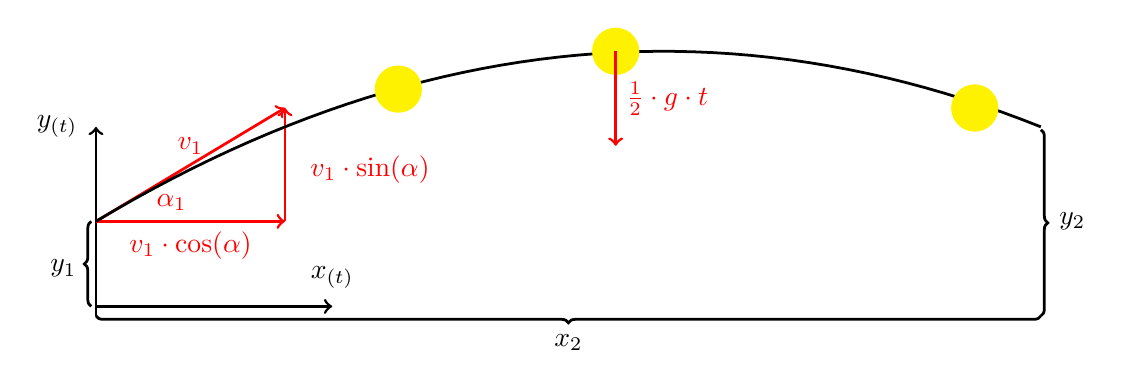
\begin{tikzpicture}[thick,scale=1.2, every node/.style={scale=1}]
        \draw[line width=1pt, decorate, decoration=brace](10, 0) -- (0, 0) (5,0)node 
        [below=1mm]{$x_2$};
        \draw[line width=1pt, decorate, decoration=brace](10, 1.97) -- (10, 0) 
        (10,1) node [right=1mm]{$y_2$};
        \draw[line width=1pt, ->](0, 0) -- (0, 2) node [left=1mm]{$y_{(t)}$};
        \draw[line width=1pt, decorate, decoration=brace](-0.5mm, 1mm) -- 
        (-0.5mm, 1) (3.2mm,0.5) node [left=5mm]{$y_1$};
        \draw[line width=1pt, ->](0, 1mm) -- (2.5, 1mm)  node [above=1mm]{$x_{(t)}$};
        \draw[line width=1pt,red, ->](0, 1) -- node[below]{$v_1 \cdot \cos(\alpha)$} 
        (2, 1);     
        \draw[line width=1pt,red, ->](2, 1) -- (2, 2.2); \node[red] at (2.9,1.55)
        {$v_1 \cdot \sin(\alpha)$}; 
        \draw[line width=1pt,red, ->](0, 1) -- node[above]{$v_1$} (2, 2.2);   
        \draw[line width=1pt,samples=50] plot [domain=0:10](\x,{-1/20*pow(\x-6,2)+2.8});
        \node[red] at (0.8,1.2){$\alpha_1$};
        \fill[yellow] (3.2,2.4) circle (0.25); 
        \fill[yellow] (5.5,2.8) circle (0.25); 
        \fill[yellow] (9.3,2.2) circle (0.25);
        \draw[line width=1pt,red, ->](5.5,2.8) -- node[right]{$\frac{1}{2} \cdot g 
        \cdot t$} (5.5,1.8); 
    \end{tikzpicture}
    \caption{Wurfparabel mit den angreifenden Kräfte}
    \label{fig:WurfparabelKraefte}
\end{figure}

\newpage
\textbf{Berechnungswerte}\\
\begin{tabular}{ll}
    \rule{0pt}{11pt} $\alpha_1$ & $45^\circ$ \\
    \rule{0pt}{11pt} $y_1$ & $0.125 m$ \\
    \rule{0pt}{11pt} $y_2$ & $0.0 m$ \\
    \rule{0pt}{11pt} $x_2$ & $1.8 m$ \\
\end{tabular}\\
\\
\\
\textbf{Resultate}\\
\begin{tabular}{ll}
    \rule{0pt}{11pt} $t$ & $0.56 s$ \\
    \rule{0pt}{11pt} $v_1$ & $4.56 \frac{m}{s}$ \\
\end{tabular}\\
\\
\\
Um den Wurf beurteilen zu können wurde dieser in der Abbildung \ref{fig:Wurfparabel} 
grafisch dargestellt.
\begin{figure}[h!]
    \centering
    \includegraphics[width=1\textwidth,clip,trim=7mm 7mm 7mm 0mm]
    {Enddokumentation/Anhang/Bilder/Schiefer_Wurf.jpg}
    \caption{Wurfparabel}
    \label{fig:Wurfparabel}
\end{figure}\\
%\newpage
Mithilfe der Abwurfgeschwindigkeit kann die Nenndrehzahl durch die Formel 
\ref{equ:v_1} definiert werden.
\begin{equation}  
    n_1 = \frac{v_1}{4\pi \cdot R_s \cdot \cos(\alpha_{Grenz})}
    \label{equ:v_1}
\end{equation}
\newpage
\textbf{Berechnungswerte}\\
\begin{tabular}{ll}
    \rule{0pt}{11pt} $R_s$ & $0.04 m$ \\
    \rule{0pt}{11pt} $\alpha_{Grenz}$ & $16.26^\circ$ \\
    \rule{0pt}{11pt} $v_1$ & $4.56 \frac{m}{s}$ \\
\end{tabular}\\
\\
\\
\textbf{Resultat}\\
\begin{tabular}{ll}
    \rule{0pt}{11pt} $n_1$ & $9.45 \frac{1}{s}$ \\
\end{tabular}\\
\\
Mit den Formeln \ref{equ:Energiegleichung} bis \ref{equ:v_1} kann die Nenndrehzahl gerechnet werden.
\begin{equation}
    m_{Ball} \cdot g \cdot \Delta h + \frac{1}{2} \cdot m_{Ball} \cdot \left[4\pi 
    \cdot R_s \cdot n_1 \cdot \cos(\alpha_{Grenz})\right]^2 + 2 \cdot J \cdot \pi^2 
    \cdot \left(n_1^2-\cdot n_0^2\right) = 0
\end{equation}

\textbf{Berechnungswerte}\\
\begin{tabular}{ll}
    \rule{0pt}{11pt} $m_{ball}$ & $0.055 kg$ \\
    \rule{0pt}{11pt} $g$ & $9.81 \frac{N}{kg}$ \\
    \rule{0pt}{11pt} $\Delta h$ & $0.01465 m$ \\
    \rule{0pt}{11pt} $R_s$ & $0.040 m$ \\
    \rule{0pt}{11pt} $n_1$ & $9.45\frac{1}{s}$ \\
    \rule{0pt}{11pt} $J$ & $0.00018 kgm^2$ \\
    \rule{0pt}{11pt} $\alpha_{Grenz}$ & $16.26^\circ$ \\
\end{tabular}\\
\\
\\
\textbf{Resultat}\\
\begin{tabular}{ll}
    \rule{0pt}{11pt} $n_0$ & $15.89 \frac{1}{s}$ \\
\end{tabular}\\
\begin{equation}
    \frac{n_1}{n_0} = 0.4 \label{equ_Prozentwert}
\end{equation}
Bei dem zurzeit vorhandenen Trägheitsmoment (Vollwelle) wird die Drehzahl um 40\% 
abgebremst. Die dabei verlorene Energie muss vom Motor zugeführt werden. 
Die Zeitdauer dafür berechnet sich wie folgt.
\begin{align}
    M_{Motor} &= \omega \cdot J \\
    n_0 &= n_1 + \omega \cdot t \\
    t &= \frac{n_0 - n_1}{\omega} = \frac{J \cdot \left(n_0 - n_1\right)}{M_{Motor}}
\end{align}

\textbf{Berechnungswerte}\\
\begin{tabular}{ll}
    \rule{0pt}{11pt} $n_0$ & $15.89 \frac{1}{s}$ \\
    \rule{0pt}{11pt} $n_1$ & $9.45 \frac{1}{s}$ \\
    \rule{0pt}{11pt} $J$ & $0.00018 kgm^2$ \\
    \rule{0pt}{11pt} $M$ & $0.1 Nm$ \\
\end{tabular}\\
\\
\\
\textbf{Resultat}\\
\begin{tabular}{ll}
    \rule{0pt}{11pt} $t$ & $0.0116 s$ \\
\end{tabular}\\
\\
Fazit dieser Berechnungen ist, dass ein erhöhtes Trägheitsmoment, die Schwungräder 
weniger abbremst, und ein grösseres Drehmoment diese schneller wieder auf die 
Nenndrehzahl beschleunigt. 
